\section{Casos de Uso}
En esta sección se describen los casos de uso del sistema propuesto, los cuales representan las principales interacciones entre el usuario y la solución de navegación asistida desarrollada. Los casos de uso permiten identificar las funcionalidades clave del sistema desde una perspectiva externa, enfocándose en las acciones que el usuario puede realizar y las respuestas que el sistema proporciona.

El sistema está diseñado para asistir a personas con discapacidad visual durante su desplazamiento en entornos urbanos o interiores, mediante la generación de instrucciones auditivas, la detección de obstáculos y la adaptación dinámica de rutas. En este contexto, los casos de uso modelan el flujo de interacción necesario para lograr una navegación segura y eficiente.

Los actores principales identificados son el \textbf{usuario}, quien interactúa mediante comandos de voz, y el \textbf{sistema}, el cual procesa la información del entorno y genera las respuestas correspondientes. A partir de esta interacción, se definen los distintos escenarios funcionales que permiten cumplir con los objetivos del sistema.
Los casos de uso considerados son los siguientes:
\subsubsection{Activar el sistema} 
Este caso de uso permite iniciar el funcionamiento del sistema de navegación mediante la activación del dispositivo.
El usuario presiona el botón de activación, el sistema se inicia, se activan los sensores, cámara y el modulo de reconocimiento de voz, el sistema queda listo para recibir instrucciones y el resultado esperado es que el sistema queda preparado para comenzar la navegación.
\subsubsection{Detener la navegación}
Permite finalizar el proceso de navegación y detener las instrucciones auditivas emitidas por el sistema.
El usuario solicita detener la navegación, el sistema cancela la ruta activa
y la navegación finaliza correctamente.
\subsubsection {Indicar destino}
El usuario proporciona al sistema el lugar al que desea dirigirse.
El usuario menciona el destino mediante comandos de voz, el sistema procesa la información recibida, identifica el destino solicitado, el sistema procede a la confirmación del destino. Así, el sistema obtiene correctamente el destino deseado.
\subsubsection {Confirmar destino}
El sistema valida que el destino interpretado sea correcto antes de iniciar la navegación.
El sistema comunica el destino detectado, el usuario confirma la información,
si la información es correcta, empieza la navegación.
\subsubsection {Emitir instrucciones de navegación}
El sistema proporciona instrucciones auditivas durante el recorrido hacia el destino seleccionado.
El sistema calcula la ruta, se generan instrucciones de navegación y el usuario recibe indicaciones auditivas. El resultado esperado es que el usuario recibe orientación continua durante el trayecto.
\subsubsection {Detectar y alertar obstáculos}
El sistema detecta obstáculos durante el desplazamiento y emite alertas preventivas al usuario.
Los sensores y cámaras monitorean el entorno, el sistema identifica posibles obstáculos, se genera una alerta auditiva y el resultado esperado es que el usuario evite colisiones.
\subsubsection {Recalcular ruta}
Permite recalcular una nueva ruta cuando el camino original presenta inconvenientes.
El sistema detecta un problema en la ruta actual, se calcula una ruta alternativa o se espera el guardado de una ruta nueva y el resultado es la navegación continúa mediante una ruta alternativa segura.
\subsubsection {Confirmar nueva ruta}
El usuario valida si desea continuar mediante la nueva ruta propuesta por el sistema.
El sistema informa la existencia de una nueva ruta, el usuario acepta o rechaza la alternativa; si acepta, el sistema actualiza la navegación, el resultado es la ruta alternativa confirmada y guardada.
\subsubsection {Finalizar navegación}
El sistema informa al usuario que ha llegado correctamente al destino seleccionado.
El sistema detecta la llegada al destino, se emite una notificación auditiva y finaliza el proceso de navegación.
% SE PUEDE ESCRIBIR UN POCO DE CADA USO O SE PUEDE HACER DESPUES DE PRESENTAR EL DIAGRAMA @Thaia

\subsection{Diagrama de casos de uso}

El diagrama de casos de uso mostrado en la Figura~\ref{fig:casos_uso} representa de manera gráfica las interacciones entre el usuario y el sistema, así como la relación entre los distintos casos de uso identificados.

\begin{figure}[H]
    \centering
    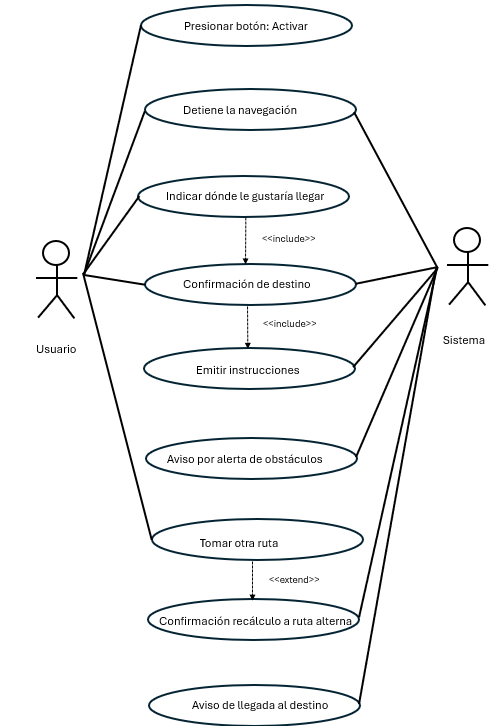
\includegraphics[width=13cm]{Diagramas/DiagCasoUso.png}
    \caption{Diagrama de casos de uso del sistema de navegación asistida}
    \label{fig:casos_uso}
\end{figure}

Este modelo permite identificar de forma clara las funcionalidades del sistema, así como las dependencias y comportamientos alternativos que pueden surgir durante su operación.
\\
El actor principal es el Usuario, quien interactúa directamente con el sistema mediante distintas funcionalidades. Por su parte, el Sistema actúa como el ente que procesa la información, toma decisiones y proporciona retroalimentación.

El usuario tiene la capacidad de activar el sistema “Presionar botón: Activar”. Este caso de uso representa la acción inicial que habilita la interacción con el sistema. Asimismo, el usuario puede detener la navegación en cualquier momento a través del caso de uso “Detiene la navegación”, lo que evidencia que el sistema debe permitir el control total sobre su ejecución.

“Indicar dónde le gustaría llegar”, donde el usuario proporciona el destino deseado. Este caso de uso describe una interacción directa en la que el sistema debe ser capaz de recibir y procesar la entrada del usuario. Asociado a este, se encuentra el caso de uso “Confirmación de destino”, el cual corresponde a una responsabilidad del sistema: validar y confirmar la información recibida. La relación <<include>> entre ambos indica que la confirmación es un comportamiento obligatorio que forma parte del servicio principal de captura de destino.

Una vez que el destino ha sido definido, el sistema ofrece la funcionalidad de “Emitir instrucciones”, que consiste en proporcionar indicaciones al usuario para llegar a su destino. Este caso de uso también está relacionado mediante <<include>>, lo que indica que depende de la confirmación previa del destino para ejecutarse correctamente.

Durante la interacción, el sistema incluye la capacidad de “Aviso por alerta de obstáculos”, lo cual representa una funcionalidad autónoma del sistema orientada a la seguridad del usuario. En este caso, el usuario no necesariamente inicia la acción, sino que el sistema actúa de manera proactiva notificando eventos relevantes del entorno.

“Tomar otra ruta”, está asociado a una relación <<extend>> con “Confirmación recálculo a ruta alterna”. Esta relación indica que se trata de una funcionalidad opcional que solo se activa bajo ciertas condiciones, como la detección de obstáculos o cambios en el entorno. En este contexto, el sistema asume la responsabilidad de recalcular una nueva ruta, mientras que el usuario participa de forma indirecta al recibir la confirmación de dicho ajuste.

El caso de uso “Aviso de llegada al destino”, representa la notificación al usuario de que se ha cumplido el objetivo de la navegación. Este caso de uso corresponde completamente al sistema, quien debe identificar el cumplimiento de la meta y comunicarlo oportunamente.